\section{Completed constrained reconstruction pairs}
All saved completed updates satisfy the common feasibility and Armijo checks. The three complete pairs reach the shared 18-update cap. Their complete-volume material errors, measured and held-out data errors, and total child walls are reported in Table~\ref{tab:supp-nonlinear}. The near-contact real component worsens slightly even while data errors decrease. This is a useful separation between local full-model fidelity and estimator quality.

\begin{table}[htbp]\centering\small
\caption{Nonlinear endpoints: unchanged receiver $\to$ verified exchange. Each wall measurement includes its own setup, acquisition, outer work, rejection and terminal evaluation; it is one trajectory timing, not a timing confidence interval.}\label{tab:supp-nonlinear}
\begin{tabular}{lrrr}\toprule
Quantity&Smooth / voxel&Near-contact / Gaussian&Shell / Gaussian\\\midrule
Complex-material error&$.30266\to.26986$&$.67219\to.67068$&$.60964\to.56599$\\
Real-material error&$.28114\to.25156$&$.68104\to.68346$&$.60815\to.56506$\\
Imaginary-material error&$.74388\to.65064$&$.44390\to.28589$&$.69755\to.62190$\\
Measured-data error&$.006637\to.002837$&$.010532\to.007083$&$.014179\to.012178$\\
Held-out data error&$.006637\to.002836$&$.010521\to.007080$&$.014190\to.012179$\\
Child wall (s)&$216.46\to579.89$&$407.71\to710.49$&$405.90\to592.29$\\
Wall ratio&2.679&1.743&1.459\\
Full-forward RHS&$354\to390$&$696\to762$&$690\to552$\\
Full-adjoint RHS&$108\to108$&$108\to108$&$108\to108$\\
Full tangent $Jx$ RHS&$0\to108$&$0\to108$&$0\to108$\\
Full tangent $Jd$ RHS&$0\to600$&$0\to636$&$0\to636$\\\bottomrule
\end{tabular}
\end{table}

The fourth object's exchange trajectory saves 17 completed accepted updates. Before update 18, construction of that trajectory's receiver-derived starting endpoint fails the frozen normal-residual test. The separate receiver-only job is not run after this fault. Thus there are six completed trajectories, one failed trajectory with a verified prefix, and one not-run baseline among eight planned jobs. No final paired material comparison is inferred for this object.

\begin{figure}[htbp]\centering
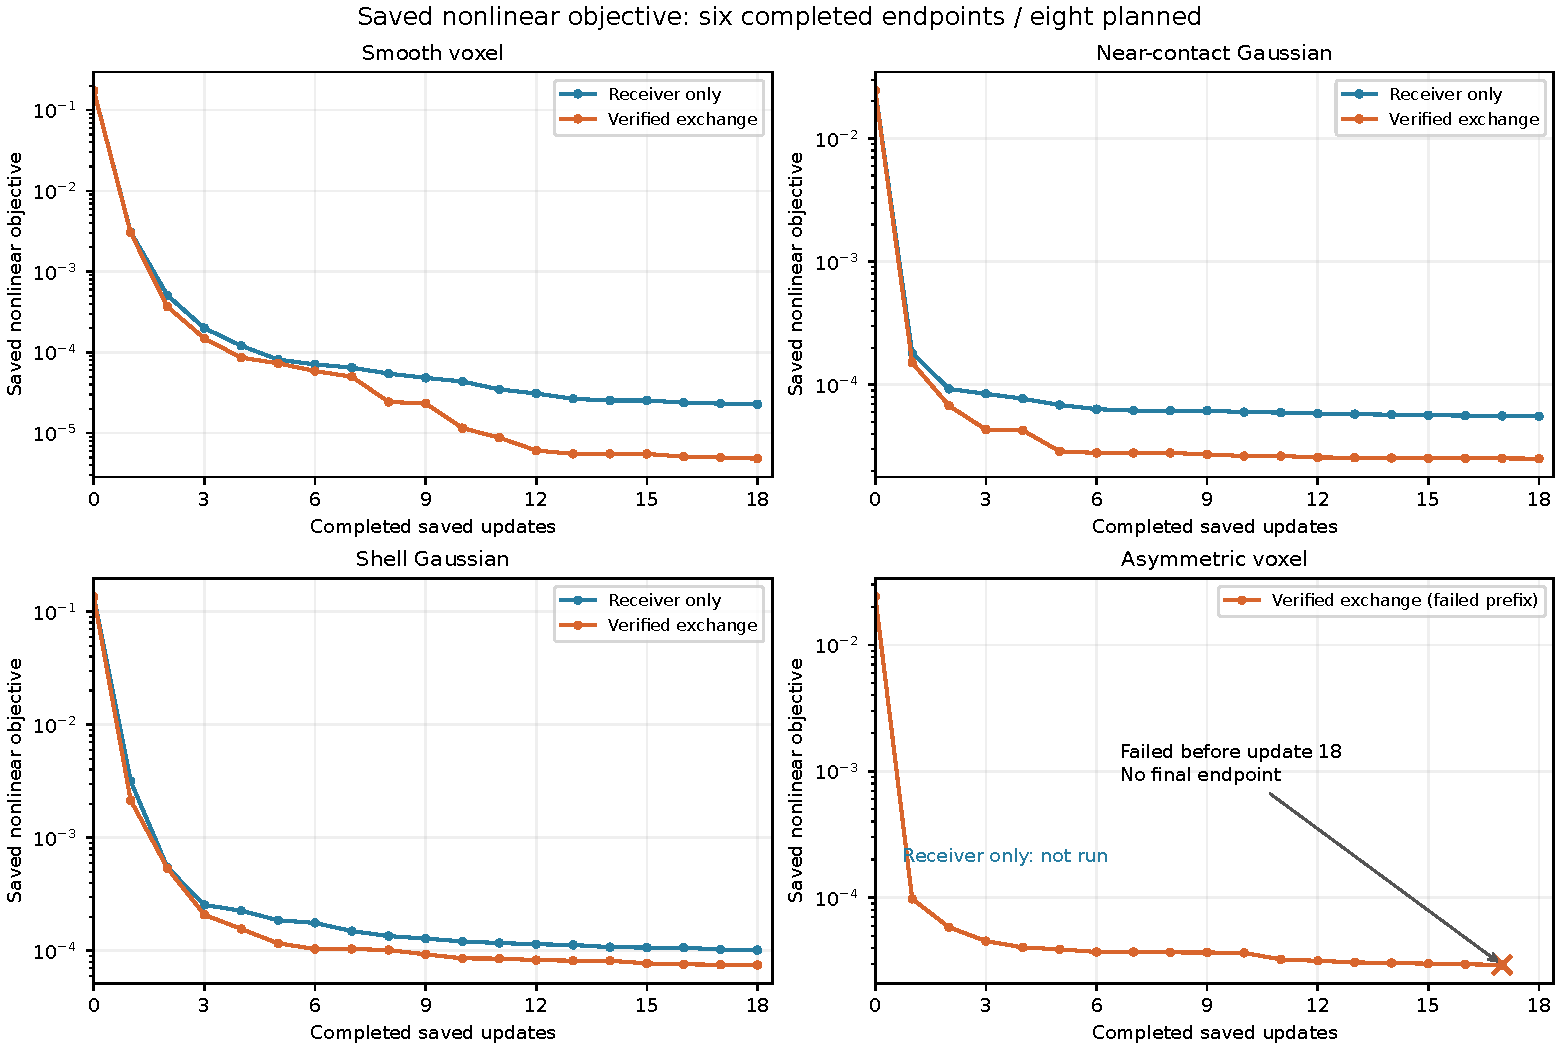
\includegraphics[width=.93\linewidth]{figures/nonlinear_closure_v1/nonlinear_objective_curves.pdf}
\caption{Accepted nonlinear objectives for the three complete pairs and the separate fourth-object prefix. The latter has no completed receiver-only comparator. Its failure and the unrun baseline remain in the eight-job denominator.}
\end{figure}

\section{Offline initial opportunity and bounded paths}
The declared initial domain contains $k(154-k)$ replacements: 600, 1168, and 2208 at $k=4,8,16$. All feasible endpoints are labeled in the 96 available cells. The 2016 late-state prerequisite exclusion leaves three unrun cells in the 99-cell denominator. Teacher labels never enter proposal, ranking, acceptance, or threshold selection.

For each complete object, we sum the positive full-dictionary best gain over its nine initial cells. Dividing the sum of anchor top-one verified/no-op gains by this denominator measures ranking capture. Dividing the sum of best gains achievable within the fixed incoming pool measures candidate coverage. Ranking capture ranges from 0.97302 to 0.99985, with median 0.99538; short-pool coverage ranges from 0.49119 to 0.95307, with median 0.72951. These are weighted one-decision opportunities, not deployed trajectory improvement fractions. The incomplete object is displayed with its observed six-cell scope and is excluded from ten-complete-object summaries.

\begin{figure}[htbp]\centering
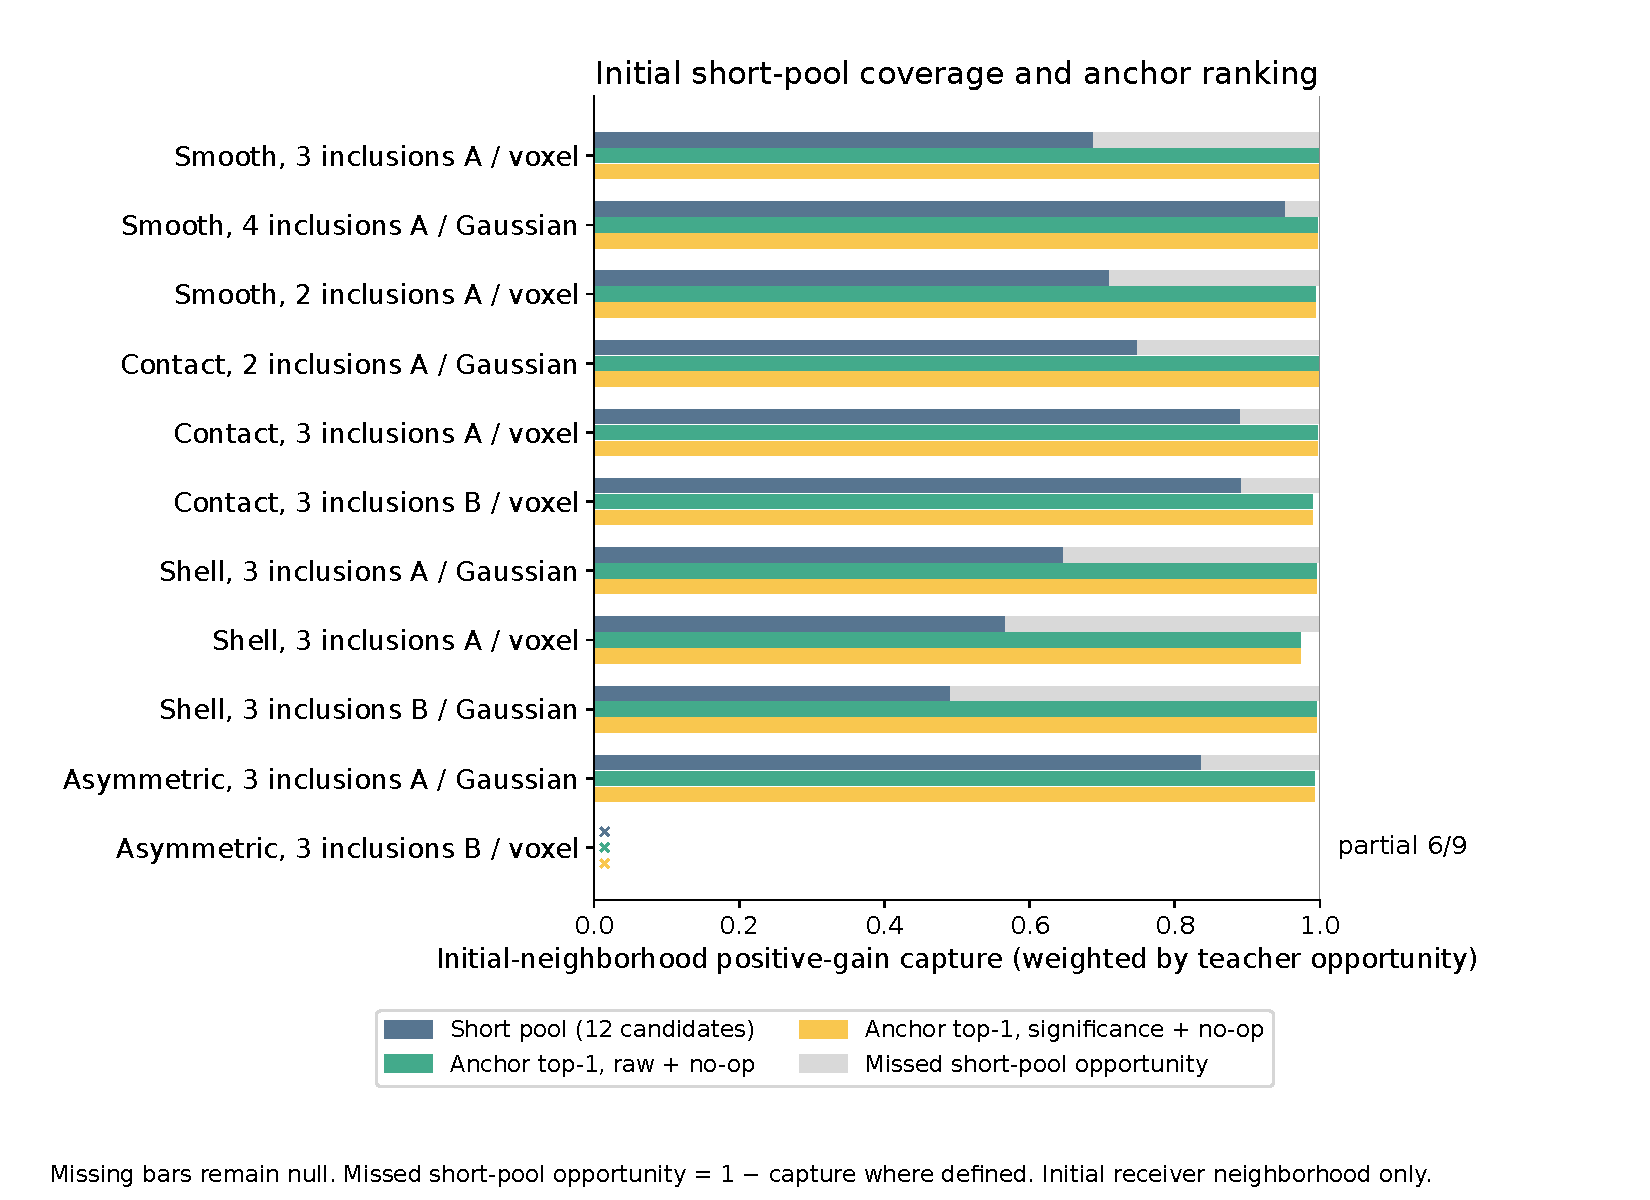
\includegraphics[width=.94\linewidth]{figures/coverage_closure_v2/initial_opportunity.pdf}
\caption{Initial receiver-neighborhood opportunity, separating reduced ranking from acquisition into the frozen 12-atom pool. Missing cells are not imputed.}
\end{figure}
\begin{figure}[htbp]\centering
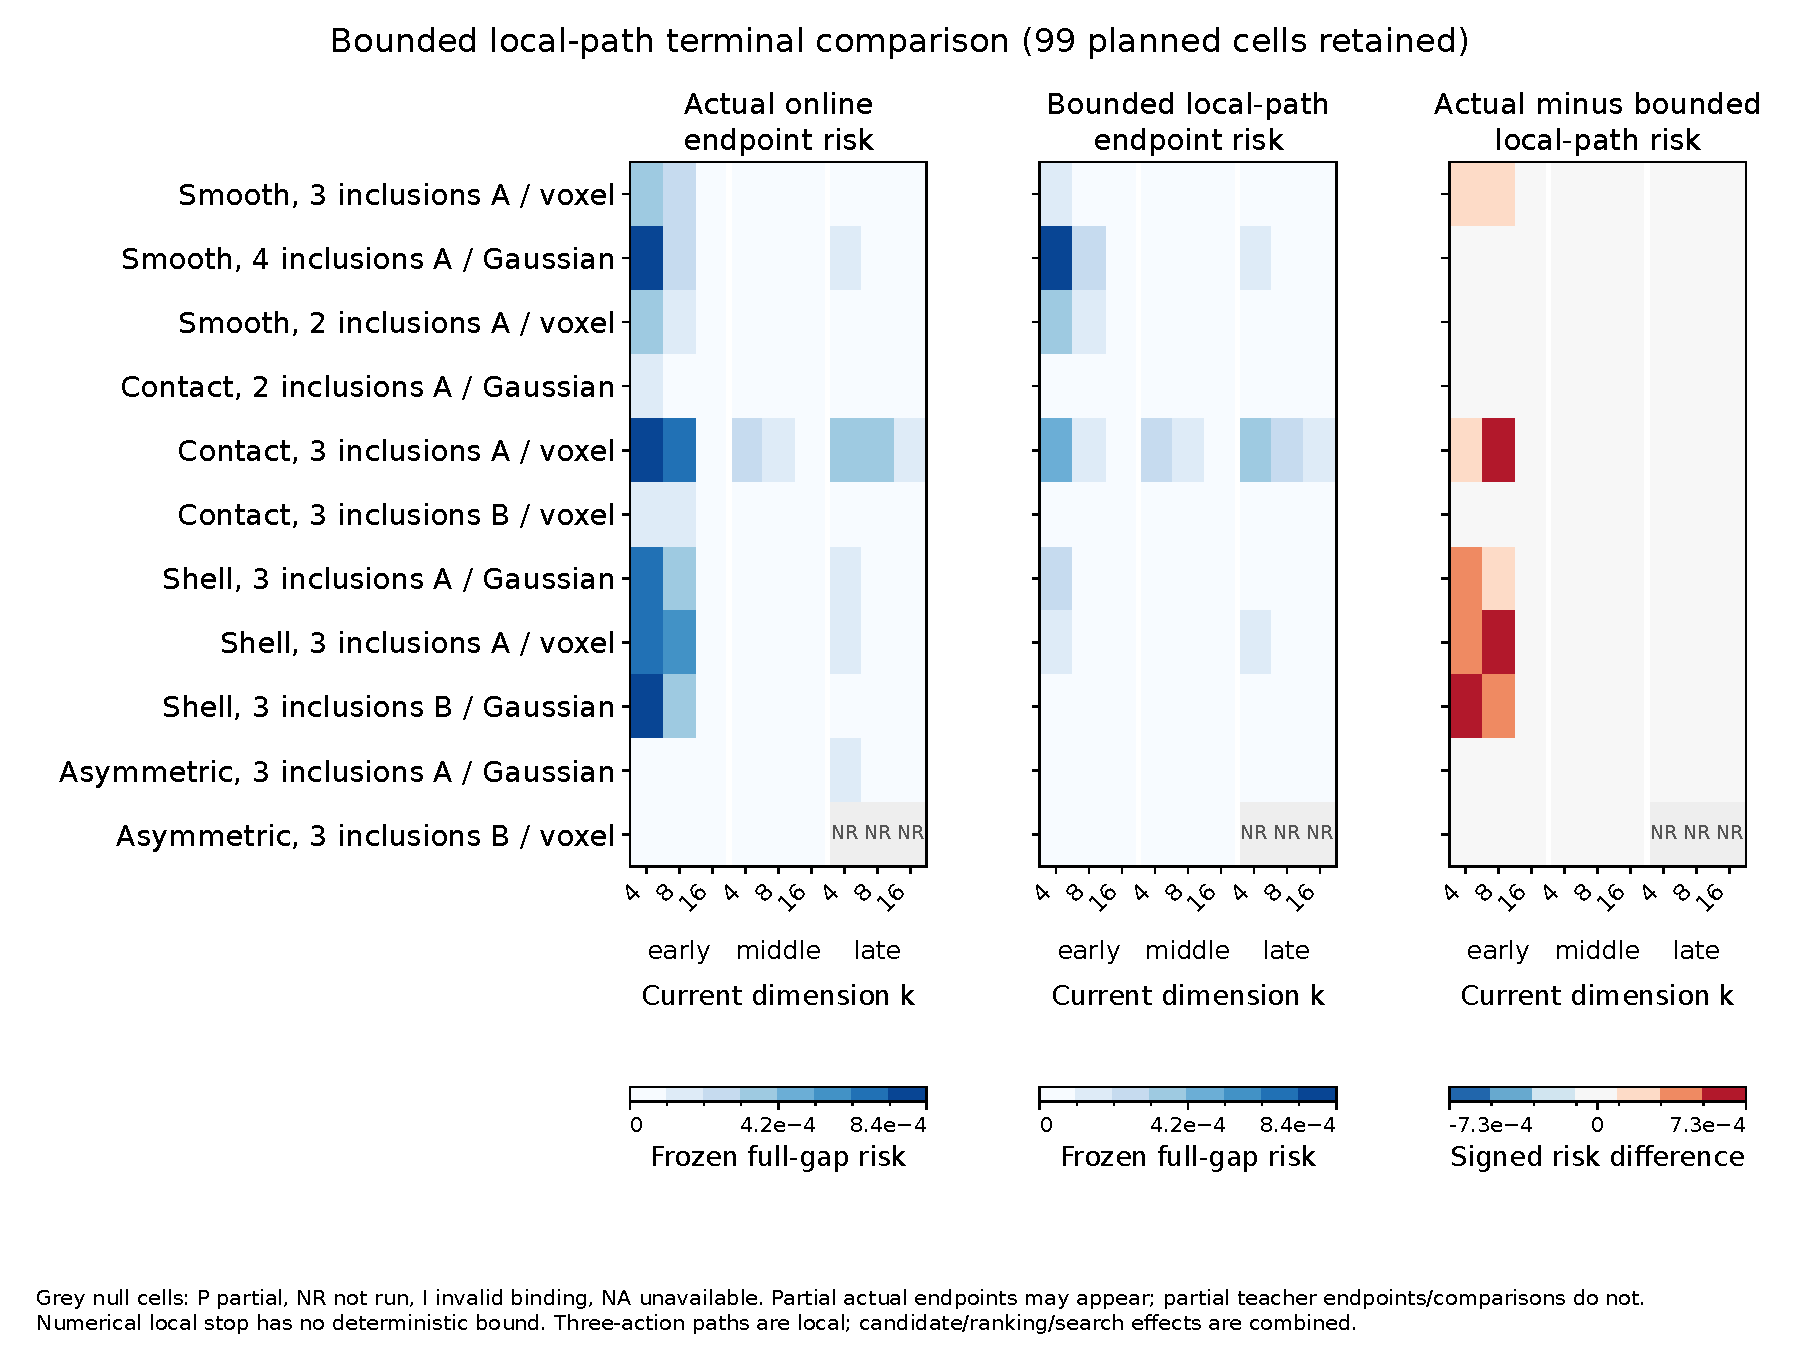
\includegraphics[width=.98\linewidth]{figures/coverage_closure_v2/bounded_path_risk.pdf}
\caption{Online and offline bounded-path final gaps. The teacher recomputes a full local one-swap neighborhood at each accepted step and stops after at most three actions. It is not a global oracle. Five online paths outperform the greedy teacher path, 90 teacher paths outperform deployment, and one differs only within the evaluation floor. These comparisons combine candidate coverage, ranking, and search interactions.}
\end{figure}


\section{Closed costs and physical-action scope}
The authoritative final ledger has 61 closed attempts with matched start/end records, comprising 57 zero and four nonzero exits. All four failed attempts retain their fees. The only additive quantities are historical carry 4889.515~s, closure occupation 15072.343~s and rejected preflight 0.202~s: total 19962.060~s. Successful preflights, child walls and A--I stage walls are already nested inside those occupation intervals.
\begin{table}[htbp]\centering\small
\caption{Mutually exclusive campaign fees. Offline diagnostics are not online deployment work.}\label{tab:closed-cost}
\begin{tabular}{lr}\toprule
Scope&Occupied wall (s)\\\midrule
Historical carry&4889.515\\
Physical threshold replay&268.749\\
Additional frozen objects&1158.673\\
Noisy frozen residuals&895.250\\
Constrained nonlinear transfer&3704.671\\
Offline coverage/path diagnosis&9039.907\\
Gate and failed setup&5.093\\
Rejected preflight outside occupation&0.202\\\midrule
Total&19962.060\\\bottomrule
\end{tabular}\end{table}

Stage views distinguish common physical setup, receiver, anchor, incoming pool, endpoint/score computation, $Jx/Jd$ checks, acceptance/rejection, offline teacher/evaluation and nonlinear work. The full ledger retains missing allocations as null. Cached Gaussian teacher labels pay the dense-$J$ acquisition once; logical cached directions do not add new physical RHS. Voxel teacher directions retain actual block-solve counters. Matrix actions, uploads, SVD, ordinary adjoint and full-adjoint counts remain distinct.

Shared frozen setup was not independently repeated as a cold receiver-only timing. Thus no cold incremental wall is manufactured by allocating a common cache to individual candidates. The three nonlinear pairs independently pay their own setup and are timed once each; their child-wall differences are 363.44, 302.77 and 186.39~s. Rejected finalists and the incomplete fourth trajectory remain charged. The maximum monitored device usage, 2692~MiB, includes other device activity and is not a policy-specific allocated-memory estimate.

